% T4 family (b): a DATA-TENSOR framework figure — the shape for problems whose
% object is a 3-D array (spatiotemporal data, multi-sensor x time x unit) that
% gets factorized / completed. Distilled in framework-figures.md from
% xinychen/awesome-latex-drawing's tensor examples.
%
% Build:  pdflatex tensor_framework_hero.tex   ->  tensor_framework_hero.pdf
% Paper:  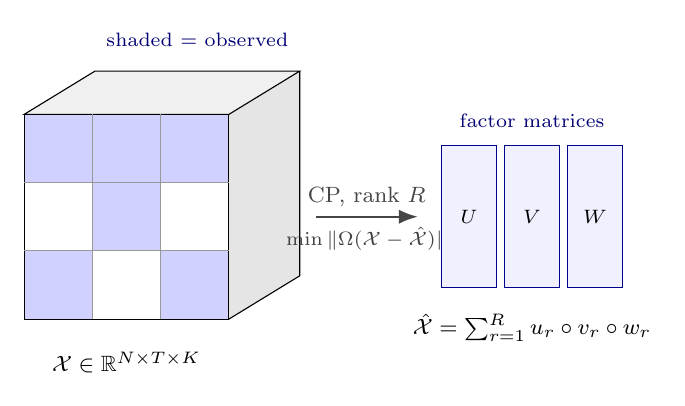
\includegraphics[width=.8\linewidth]{tensor_framework_hero.pdf}
%
% Technique: a parametrized 3-D block (\tW,\tH,\tDx,\tDy iso offset) drawn as a
% plain-TikZ parallelepiped — robust, no extra package. (tikz-3dplot generalizes
% this to arbitrary camera rotation if you need it.) The "real method object" is
% the partially-observed tensor itself (shaded = observed, white = missing),
% factorized into CP factor matrices. NB: \W/\H are taken by LaTeX accents, so
% the block dims use a \t- prefix.
\documentclass[border=3mm]{standalone}
\usepackage{tikz}
\usepackage{amsmath, amssymb}
\usetikzlibrary{arrows.meta, calc, positioning}
\newcommand{\tW}{2.6}\newcommand{\tH}{2.6}\newcommand{\tDx}{0.9}\newcommand{\tDy}{0.55}
\begin{document}
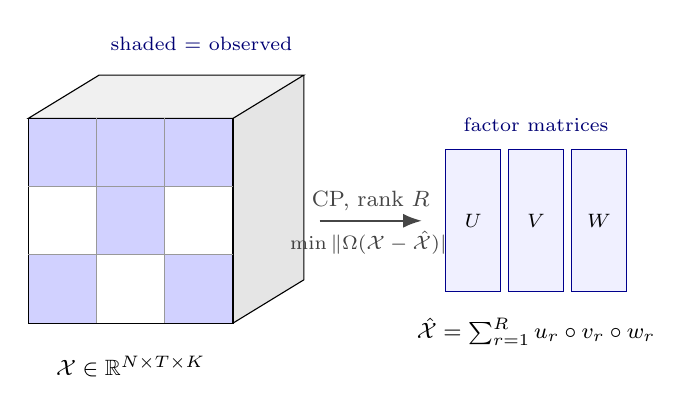
\begin{tikzpicture}[
  arr/.style={-{Latex[length=2.4mm]}, thick, gray!55!black},
  fac/.style={draw=blue!55!black, fill=blue!6},
  font=\small,
]
  % ===================== data tensor X (partially observed) =================== %
  % top and right faces (context), then a gridded, partly-shaded front face
  \fill[black!6]  (0,\tH) -- (\tW,\tH) -- (\tW+\tDx,\tH+\tDy) -- (\tDx,\tH+\tDy) -- cycle; % top
  \fill[black!10] (\tW,0) -- (\tW+\tDx,\tDy) -- (\tW+\tDx,\tH+\tDy) -- (\tW,\tH) -- cycle;  % side
  \draw (0,\tH) -- (\tW,\tH) -- (\tW+\tDx,\tH+\tDy) -- (\tDx,\tH+\tDy) -- cycle;
  \draw (\tW,0) -- (\tW+\tDx,\tDy) -- (\tW+\tDx,\tH+\tDy);
  % front face: 3x3 cells, some observed (shaded), some missing (white)
  \foreach \i/\j in {0/0, 0/2, 1/1, 2/0, 2/2, 1/2}
    \fill[blue!18] ({\i*\tW/3},{\j*\tH/3}) rectangle ({(\i+1)*\tW/3},{(\j+1)*\tH/3});
  \draw (0,0) rectangle (\tW,\tH);
  \foreach \k in {1,2}{ \draw[black!40] (\k*\tW/3,0) -- (\k*\tW/3,\tH);
                        \draw[black!40] (0,\k*\tH/3) -- (\tW,\k*\tH/3); }
  \node[font=\footnotesize] at (\tW/2,-0.55) {$\mathcal{X}\in\mathbb{R}^{N\times T\times K}$};
  \node[font=\scriptsize, text=blue!45!black] at (\tW/2+\tDx, \tH+\tDy+0.4)
        {shaded = observed};

  % ===================== factorization arrow ================================= %
  \draw[arr] (\tW+\tDx+0.2,\tH/2) --
    node[above, font=\footnotesize]{CP, rank $R$}
    node[below, font=\scriptsize, text=gray!50!black]{$\min\|\Omega(\mathcal{X}-\hat{\mathcal{X}})\|$}
    (\tW+\tDx+1.5,\tH/2);

  % ===================== CP factor matrices U, V, W =========================== %
  \begin{scope}[shift={(\tW+\tDx+1.8,0)}]
    \node[fac, minimum width=7mm, minimum height=18mm] (U)  at (0.35,\tH/2) {};
    \node[fac, minimum width=7mm, minimum height=18mm] (V)  at (1.15,\tH/2) {};
    \node[fac, minimum width=7mm, minimum height=18mm] (Wm) at (1.95,\tH/2) {};
    \node[font=\scriptsize] at (U) {$U$}; \node[font=\scriptsize] at (V) {$V$};
    \node[font=\scriptsize] at (Wm) {$W$};
    \node[font=\footnotesize, below=2mm of V]
      {$\hat{\mathcal{X}}=\sum_{r=1}^{R} u_r\circ v_r\circ w_r$};
    \node[font=\scriptsize, above=1mm of V, text=blue!45!black] {factor matrices};
  \end{scope}
\end{tikzpicture}
\end{document}
